\documentclass{article}
\usepackage[a4paper]{geometry}
\usepackage[italian]{babel}
\usepackage[parfill]{parskip}
\usepackage[utf8]{inputenc}
\usepackage{amsfonts} 
\usepackage{graphicx}
\usepackage{hyperref}
\usepackage{listings}
\usepackage{natbib}
\usepackage{xcolor}

\definecolor{codegreen}{HTML}{1E5E19}
\definecolor{codegray}{HTML}{1E5E19}
\definecolor{codepurple}{HTML}{1E5E19}
\definecolor{backcolour}{HTML}{FAFAFA}

\lstdefinestyle{mystyle}{
    backgroundcolor=\color{backcolour},   
    commentstyle=\color{codegreen},
    keywordstyle=\color{magenta},
    numberstyle=\tiny\color{codegray},
    stringstyle=\color{codepurple},
    basicstyle=\ttfamily\footnotesize,
    breakatwhitespace=false,         
    breaklines=true,                 
    captionpos=b,                    
    keepspaces=true,                 
    numbers=left,                    
    numbersep=5pt,                  
    showspaces=false,                
    showstringspaces=false,
    showtabs=false,                  
    tabsize=2
}

\title{A method to compute the expected value of the profit gainable competing in the Bitcoin Network with commercial ASIC devices\\($5^{th}$ draft)}

\author{Luca Polverini \\ email luca.polverini@gmail.com}

\date{9 February 2020}

\usepackage{natbib}
\usepackage{graphicx}

\begin{document}

\maketitle

\begin{abstract}
    In questo capitolo si descrive un metodo per il calcolo del profitto (perdita) ricavabile dall'attività di mining di cryptovaluta.
\end{abstract}

\tableofcontents

\section{Introduction}

This note shows a simple method to compute the expected value of the coin-base subsides gainable competing as a miner in the Bitcoin network.
In particular, we inspect the profitability of running ASIC devices summing to an amount of "hash rate" $h$.

Many web sites, to compute the profitability, use methods that can be misleading because they don't take into account the global hash rate growth of the Bitcoin network.

\section{Trattazione della difficoltà}

La funzione di hash SHASUM256 è una applicazione che mappa dati interi non negativi in un intero appartenente all'intervallo chiuso $ \left [0, 2^{256} - 1 \right ]$:

\begin{equation}
    h: \mathbb{Z}^{+} \cup {0} \rightarrow \{ z \in \mathbb{Z}^{+} \cup {0} \mid z  \leq 2^{256} - 1 \} \label{applicazione_hash}
\end{equation}

In Bitcoin, per produrre un blocco valido, è necessario formare una testata di blocco tale per cui l'hash della stessa dia luogo a un codice $h_{block}$ che rispetti la condizione:

\begin{equation}
    h_{block} < T \label{condizione_hash}
\end{equation}

dove $T$ è il valore target (\textit{bnTarget} in pow.cpp). In Bitcoin la difficoltà corrente è indicata nel campo nBits della testata del blocco.
Il formato del campo nBits è Compact, maggiori informazioni sono in appendice.

La difficoltà di questa ricerca è dovuta al fatto che gli hash generati nel corso della \textit{Proof of Work} sono distribuiti uniformemente nell'intervallo $ \left [0, 2^{256} - 1 \right ]$ ma il valore target $T$ è molto inferiore a $2^{256} - 1$. 

Per scelta progettuale $T_{max}$, il massimo valore che $T$ può assumere, vale $2^{224} - 1$, e dunque:

\begin{equation}
    T \le T_{max} = 2^{224} - 1 \ll 2^{256} - 1 \label{target_value}
\end{equation}

La difficoltà $D$ è definita nel file blockchain.cpp e è data dalla seguente espressione:

\begin{equation}
    D = \frac{T_{max}}{T} \label{diff}
\end{equation}

La ricerca di un hash valido è una \textbf{prova di Bernoulli} che ha probabilità di successo:

\begin{equation}
    \label{eq:pbloc}
    p(h_{block}^{(i)} < T) = \frac{T}{2^{256}} =\frac{T_{max}}{D \cdot 2^{256}} = \frac{1}{2^{32} \cdot D}
\end{equation}

dove $i$ rappresenta l'i-esimo tentativo.

Dalla (\ref{eq:pbloc}), si evince che la massima probabilità possibile è data da $D = 1$ e vale $p = 2^{-32}$.

La distribuzione di probabilità del numero di tentativi $k$ necessari per per ottenere un hash valido è data dalla distribuzione geometrica:

\begin{equation}
    P(X = k) = (1 - p)^{k-1} \cdot p^{1} \label{distribuzione_geometrica}
\end{equation}

per $k \in \mathbf{Z}^{+}$

La distribuzione geometrica ha valore atteso e varianza date dalle seguenti espressioni

\begin{equation}
    \mathbb{E}(X) = p^{-1} = \frac{2^{256}}{T} \label{valore atteso}
\end{equation}

Dal quale si ricava che il numero medio di tentativi necessari è molto ampio ed ha varianza $\approx \frac{1}{p^{2}}$:

\begin{equation}
    \sigma^{2}(X) = \frac{1 - p}{p^2} \label{varianza}
\end{equation}

In data odierna, i valori sono i seguenti:

\begin{equation}
    \left \{
        \begin{array}{ll}
            D = 1.55 \cdot 10^{13} \\
            p = 1.51 \cdot 10^{-23} \\
            \mathbb{E}(X) = 6.64 \cdot 10^{22}\\
            \sigma^{2}(X) = 4.41 \cdot 10^{45}
        \end{array}
    \right  \}
\end{equation}

Un processo di arrivi di Poisson è un processo stocastico utile per modellare gli arrivi in un sistema. Può essere visto come la versione continua di un processo di Bernoulli. Per un processo di Bernoulli gli arrivi possono verificarsi soltanto in corrispondenza in multipli interi di un incremento dato.

In un processo di Poisson gli arrivi possono verificarsi arbitrariamente e la probabilità di un arrivo per ogni particolare istante è nulla. 
Ciò significa che non esiste un modo per descrivere la probabilità di arrivo in un punto ed è più facile riferirsi a sequenze di arrivi in un intervallo; tali sequenze sono quantità i.i.d.

In letteratura la ricerca \textit{Proof of Work} è spesso ritenuta modellabile con sufficiente approssimazione attraverso un processo di Poisson di parametro $\lambda$.

Se la variabile casuale $X$ rappresenta il numero di arrivi in un intervallo di tempo $t$, indipendente dall'origine dei tempi, sotto le le ipotesi:

\begin{itemize}
    \item uniformità
    \item indipendenza e assenza di memoria
    \item ordinarietà
\end{itemize}

la densità si distribuisce come una variabile casuale di parametro $\lambda = r \cdot t$.

\begin{equation}
    r = \frac{h}{2^{32}D} \label{rate}
\end{equation}

\begin{equation}
    \lambda = \frac{h}{2^{32}D} \cdot t \label{lambda}
\end{equation}

dove $h$ è la frequenza di hash $(\frac{H}{s})$ e $\lambda$ è il valore atteso degli arrivi nell'unità di tempo:

\begin{equation}
    \mathbb{E}_{1}(X) = \lambda \label{E_lambda}
\end{equation}

La distribuzione di probabilità (PDF) ha la seguente forma:

\begin{equation}
    f(X; t) = \lambda \cdot e^{-\lambda} = rt \cdot e^{-rt}
\end{equation}

dove $t$ è la durata della batteria di prove espresso in  secondi $(s)$.

La distribuzione di probabilità cumulativa (CDF) è data da:

\begin{equation}
    P(X; t) = 1 - e^{-rt} = 1 - e^{-\lambda} \label{eq:CDF}
\end{equation}

\subsection{Esempio}

Se $h = 1 \ GH/s$ e $D = 1690906$ la remunerazione per ogni arrivo e $t = 86400 \ s$ (1 giorno), la probabilità di arrivo in un giorno è pari a:

\begin{equation}
    \lambda = \frac{h \cdot t}{2^{32} \cdot D} = \frac{1 \cdot 10^{9} \cdot 86400}{2^{32} \cdot 1690906} \approx 0.0119
\end{equation}

Se $S_{B} = 12.5 \ BTC$ BTC, possiamo ricavare il sussidio utilizzando dalla seguente:

\begin{equation}
    S = \lambda \cdot S_{B} \label{eq:lamdaToSubside}
\end{equation}

che nel caso in esame è pari a $0.59 \ BTC$ (i valori attuali sono molto distanti da questo semplice esempio!).

La varianza del processo è ancora $\lambda$, dunque 0.0119, e la deviazione standard $\sigma = 0.109$, circa 9.17 volte superiore.

Va sottolineato che il processo è random e senza memoria.

Imponendo la (\ref{eq:CDF}) a 0.8 otteniamo il seguente valore per $t$:

\begin{equation}
    P(X; t) = 1 - e^{-\lambda \cdot t} = .80 \Rightarrow  e^{-\lambda \cdot t} = 0.20 \Rightarrow  {\lambda \cdot t} = -\ln(0.20) \Rightarrow t \approx 135 \textit{giorni!} 
\end{equation}

\section{Stima dell'hash globale del network}

Il protocollo Bitcoin adatta il valore della difficoltà $D$ ogni 2016 blocchi in maniera tale da inseguire il valore 1 blocco ogni 600 secondi.

Approssimando, è dunque possibile ricavare una stima della frequenza di hash della rete $H$.

\begin{equation}
    \lambda_{net} \cdot t = \frac{H}{2^{32}D} \cdot t = 1 \Rightarrow H = \frac{2^{32} \cdot D}{t} \label{lamda_net}
\end{equation}

per $t = 600 \ \textnormal{sec}$

\section{Riduzione della varianza mediante la partecipazione in un Pool}

La partecipazione ad un pool di mining di "potenza" $h_{\textit{pool}} = k \cdot h$ induce una varianza $\sigma_{\textit{pool}}^{2}$ $k$ volte inferiore.

Se ad esempio $K = 100$, pur mantenendo costante il valore atteso pari a 0.59 $BTC$, la $P_{pool}$ diviene

\begin{equation}
    t = -\frac{\ln(0.20)}{k \cdot \lambda} \approx 1.35 \ \textit{giorni!} 
\end{equation}

La varianza e ridotta proporzionalmente a k.

Il gestore del pool remunera la propria attività trattenendo una quota $f$ del sussidio. Gli schemi adottati sono vari, ed includono la trattazione delle commissioni. 
In questa parte assumeremo l'uso della schema PPS e trascureremo, per il momento, le parte reltiva alle commissioni.

Alcuni degli \href{https://en.bitcoin.it/wiki/Comparison_of_mining_pools}{schemi adottati} da alcuni pool possono essere consultati.

In questo scenario dovremo tenere in considerazione che il ricavato dall'attività di mining, beneficiando della riduzione di varianza,
subirà una riduzione:

\begin{equation}
    \mathbb{E} = (1 - f) \cdot \frac{h \cdot t}{2^{32} \cdot D} \label{adjusted_lambda}
\end{equation}




\lstset{style=mystyle}
\begin{lstlisting}[language=VBScript]
/* Example */
var k = 1000; // partecipanti pool
var P = .95;
var D = 15466098935554.65;
var day = 86400; // seconds
var h = 73 * Math.pow(10, 12);
var lambda = k * h / (Math.pow(2, 32) * D);
console.log("lambda pool", lambda)
var p = lambda * day;
console.log("p pool(1 day) = ", p)
var t = - Math.log(1- P) / lambda / (day);
console.log("P = ", P, "=> time = ", t, "days")
console.log("pool pay out day", p * 25 * 10000)
var BTCUSD = 9500
var b1 = p * 25 * BTCUSD / k
console.log("pay out day", b1)
var e = 24 * 2.9 * 0;
var c1 = e + 2000/365;
console.log("costs", c1)
console.log("profit per kWh", (b1 - c1)/24/2.9)
\end{lstlisting}

\begin{figure}[!htb]
    \centering
    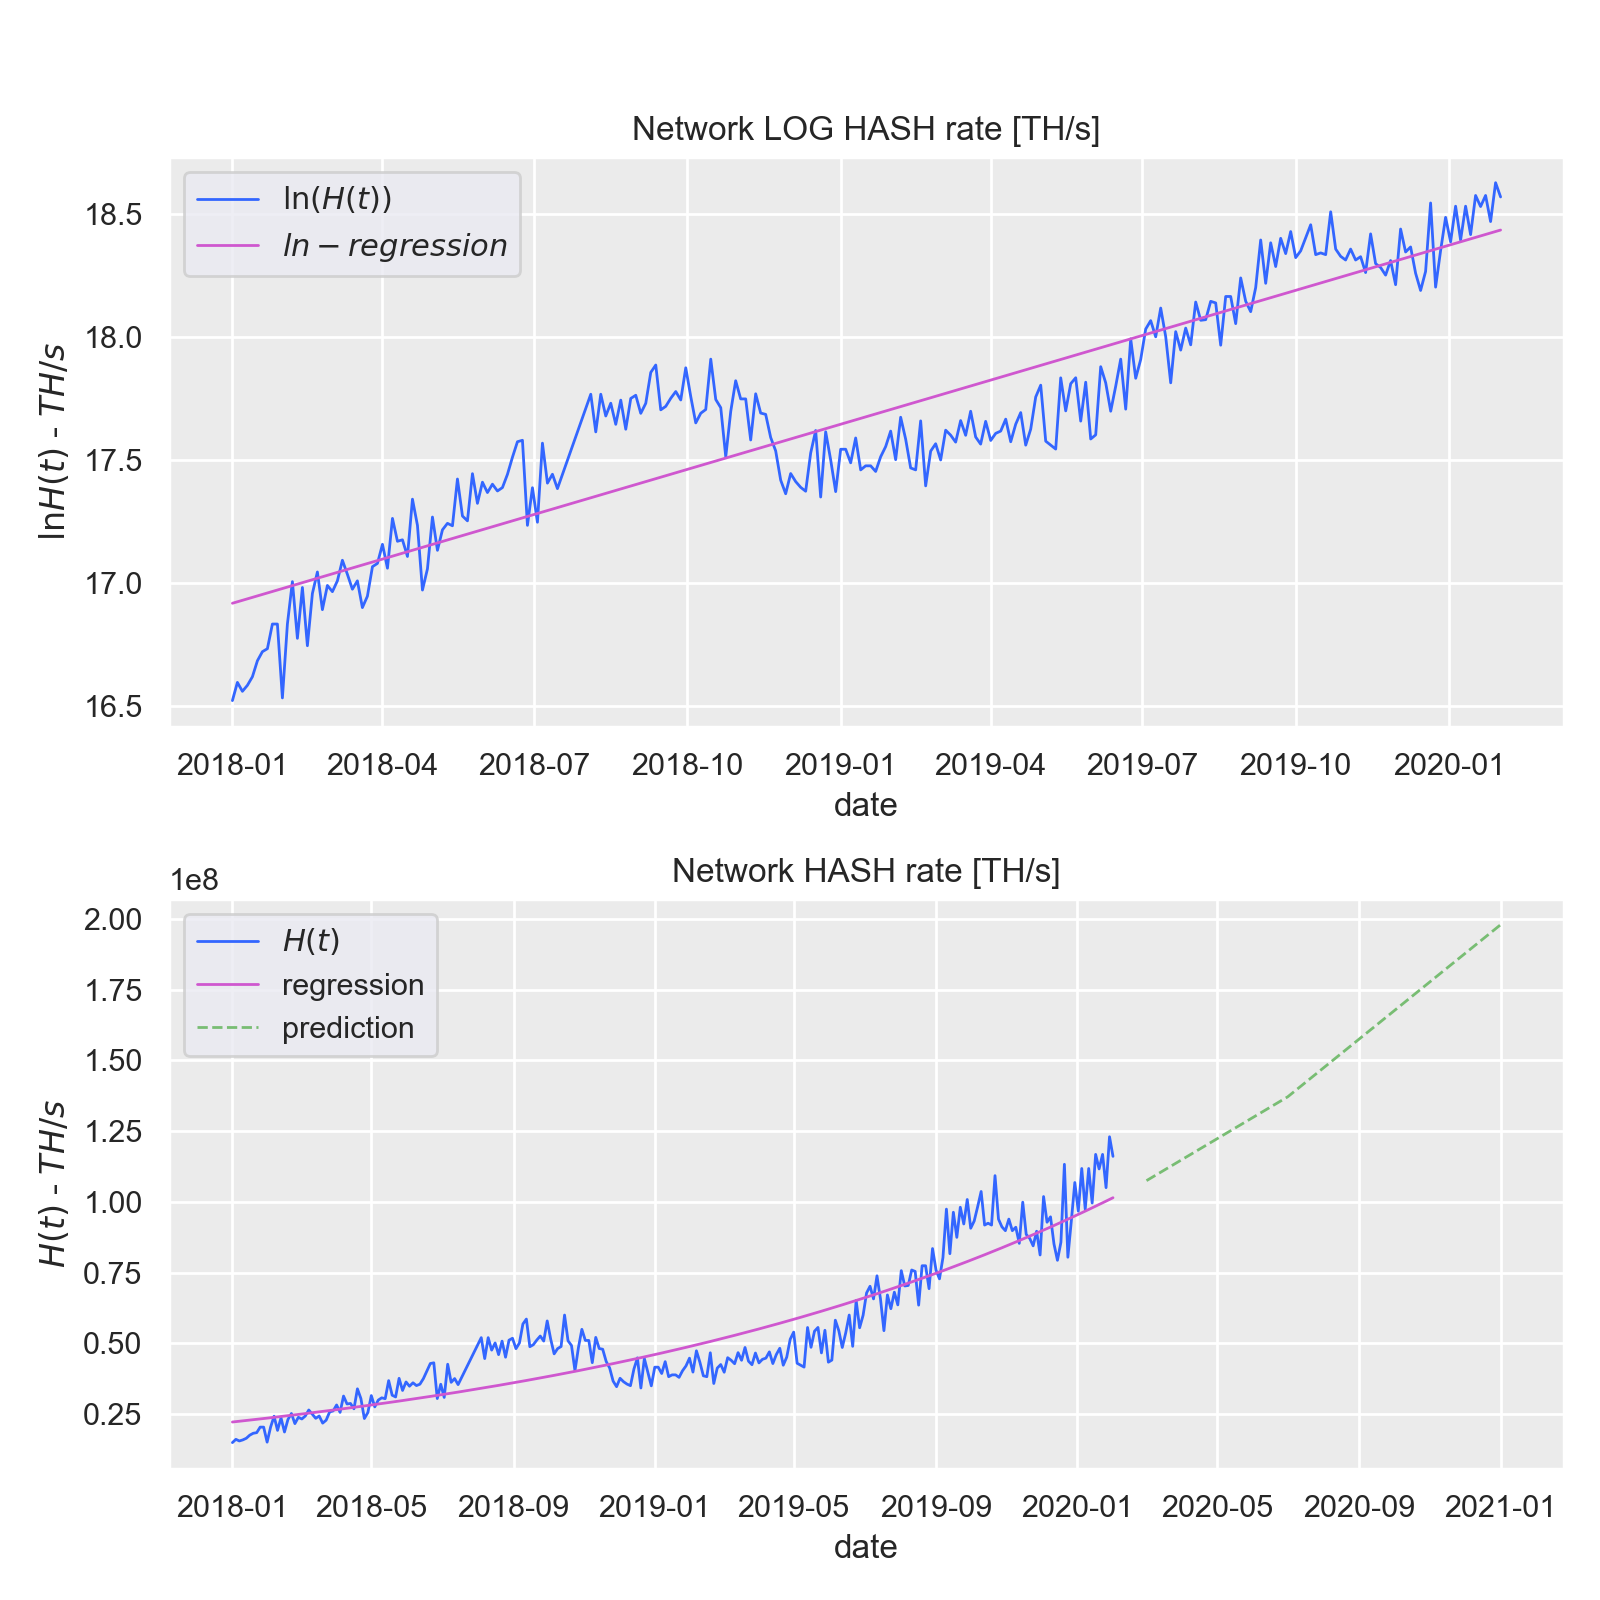
\includegraphics[width=1.0\textwidth]{img/bitcoin-hash-rate.png}
    \caption{Global log-hash rate of the Bitcoin network from Jan, 2018 to Feb, 2020.}
    \label{fig:hash_power}
\end{figure}

\section{Hash rate growth}

The global hash rate can be esteemed indirectly through the difficulty that is recorder in the block header:

\begin{equation}
    \widehat{H_{i}} = \frac{2^{32}}{600} \cdot D_{i+1} \label{H_estimate}
\end{equation}

We have downloaded the estimated global hash rate data $\widehat{H}(t)$ from the web site https://www.blockchain.com/.

The Figure (\ref{fig:hash_power}) shows the natural logarithm of the hash rate growth $\ln(H(t))$ from Jan 1, 2018 to Feb 1, 2020.

The time unit is seconds ($s$), and the format is the unix epoch, thus seconds elapsed from January 1, 1970.

The hash rate unit is tera hashes per seconds ($TH/S$).

Given the data, we have fit the data to a line using the log-linear regression:

\begin{equation}
    \ln(\widehat{H}(t)) = m \cdot t + q  \label{eq1}
\end{equation}

from which we have derived:

\begin{equation}
    \widehat{H}(t) = e^{q} \cdot e^{m \cdot t} \label{eq11}
\end{equation}

Equation (\ref{eq11}) serves as a short term predictor for future global hash rate values.\\

The regression exhibits an acceptable fitness to the data. In the future developments of this method, we will show errors and residuals.

We know that growth might rise or decline, but the behaviour is reasonably log-linear since 2014.

Fitting the data, the parameters of the equation (\ref{eq11}) are the following values:

\begin{equation}
    \left \{
        \begin{array}{ll}
            m = +2.29349988795e-08 \\
            q = -17.816879116
        \end{array}
    \right \} \label{values}
\end{equation}

\section{Probability of winning a block}

The Bitcoin protocol is coded to adjust the difficulty in such a way that the expected time to build a block is 10 minutes (600 seconds).

So we can imagine the rent-seeking competition among miners (\cite{theEconomicLimits}) to build a new block as composed of rounds of 10 minutes each.

Given the global network hash rate $H(t)$ and the hash rate owned by a single miner (or mining pool) $h(t)$, we can compute the probability $p_{win}(t)$ of gaining the subside $S_{block}$ for a single round $r(t)$ that starts at $t$ and ends at $t+600$ seconds under the assumption that all the competitors use the "same technology" and the "same algorithms".

The same algorithms assumption seems to be accepted as guaranteed by the Bitcoin protocol and by the nature of the Proof of Work and its cryptographic hash functions (the underlying probability distribution is uniform) that entitles us to consider the random variables independent and identically distributed.

The same technology assumption is weak and serves to overcome some issues related to networking and other minors and majors issues.

The probability is:

\begin{equation}
    p_{win}(t) = \frac{h(t)}{H(t)} \label{eq2}
\end{equation}

In our scenario, $h(t)$ is constant in time and it is much lower than $H(t)$: 

\begin{equation}
    h(t) = h_{o} \ll H(t) \label{eq3}
\end{equation}

So we can write:

\begin{equation}
    p_{win}(t) = \frac{h(t)}{H(t)} = \frac{h_{0}}{H(t)} \label{eq4}
\end{equation}

\section{Expectation}

We can define a random variable $X$ such that:

\begin{equation}
X = \left\{
        \begin{array}{ll}
            X = 1 \textit{, if the miner wins the round} \\
            X = 0 \textit{, if the miner loses the round}
        \end{array}
    \right \} \label{rndX}
\end{equation}

The expected value of X over $n$ rounds is:

\begin{equation}
    \mathbf{E}(X) = \displaystyle\sum_{r=1}^{n} 1 \cdot p_{win}(t(r)) + 0 \cdot ( 1 - p_{win}(t(r))) \label{eq5}
\end{equation}

Where:

\begin{equation}
    t(r) = t_{(r=1)} + 600 \cdot r \label{eq6}
\end{equation}

Rearranging the preceding equations we can write:

\begin{equation}
    \mathbf{E}(X) = \displaystyle\sum_{r=1}^{n} \frac{h0}{\widehat{H}(t(r))} \label{expectationPwinOverRounds}
\end{equation}

Given equation (\ref{expectationPwinOverRounds}) the following code follows:

\begin{lstlisting}[language=Python]
# --------------------------------------------------
# Compute the expected value of X
# --------------------------------------------------

E = 0
r = 0

while(r <= 365 * 24 * 6): # e.g. 1 year
    r += 1
    E += h0 / H(t(r))

return E
\end{lstlisting}

Or, if we want to compute the expected number of rounds needed to win a block:

\begin{lstlisting}[language=Python]
# --------------------------------------------------
# Compute the number of rounds needed to win a round
# --------------------------------------------------

E = 0
r = 0

while(E < 1): # e.g. 1 win
    r += 1
    E += h0 / H(t(r))

return r
\end{lstlisting}

\section{Results}

Given a single high-end commercial ASIC device, the hash rate is $h_{0} = 73\ TH/s$ and under our assumptions
the expected number of wins in a year, starting from Feb. 2, 2020, is:

\begin{equation}
    \mathbf{E}(X) = \displaystyle\sum_{r=0}^{365*24*6} p_{win}(t(r)) \approx 0.026 \label{res1}
\end{equation}

Obviously, given $N=100$ devices of the same model, the result is:

\begin{equation}
    \mathbf{E}(X) = \displaystyle\sum_{r=0}^{365*24*6} p_{win}(t(r)) \approx 2.58 \label{res11}
\end{equation}

\section{Economic prospects drafts}

In this paragraph, we show two simplified economic prospects.

Given the exhibited exponential growth of the global hash-rate, and given the fact that ASIC devices are not repurposable, we have decided to take into account all the device cost without amortization.

Given the BTC price fluctuation (volatility), we have also avoided taking account of interests rates.

\begin{figure}[h]
    \centering
    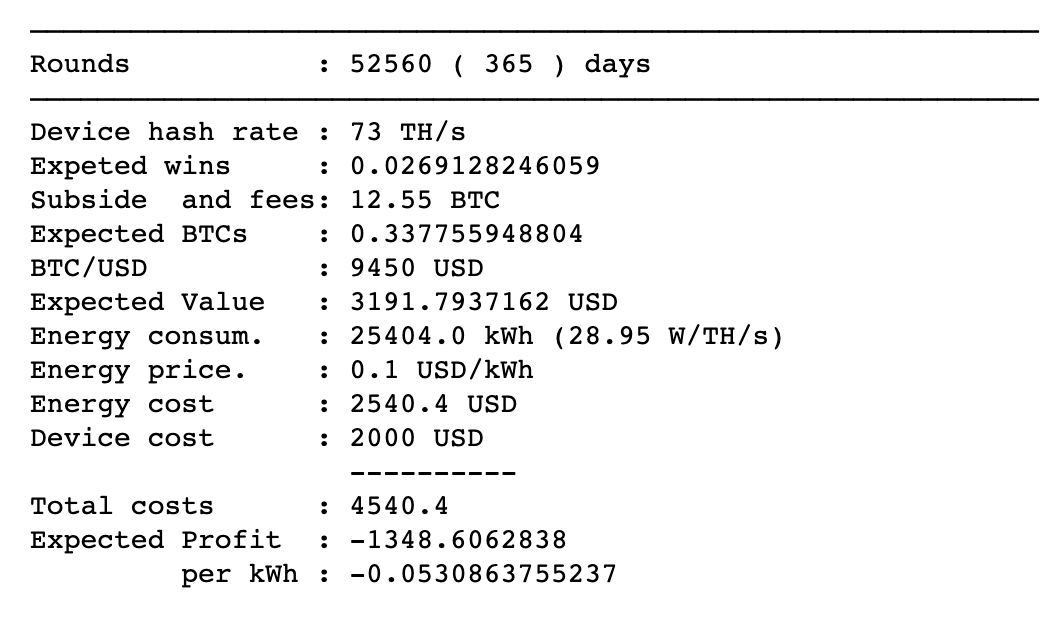
\includegraphics[scale=0.50]{img/results-12.png}
    \caption{Model results for $S = 12.5 BTC$}
    \label{fig:results-12}
\end{figure}

\begin{figure}[h]
    \centering
    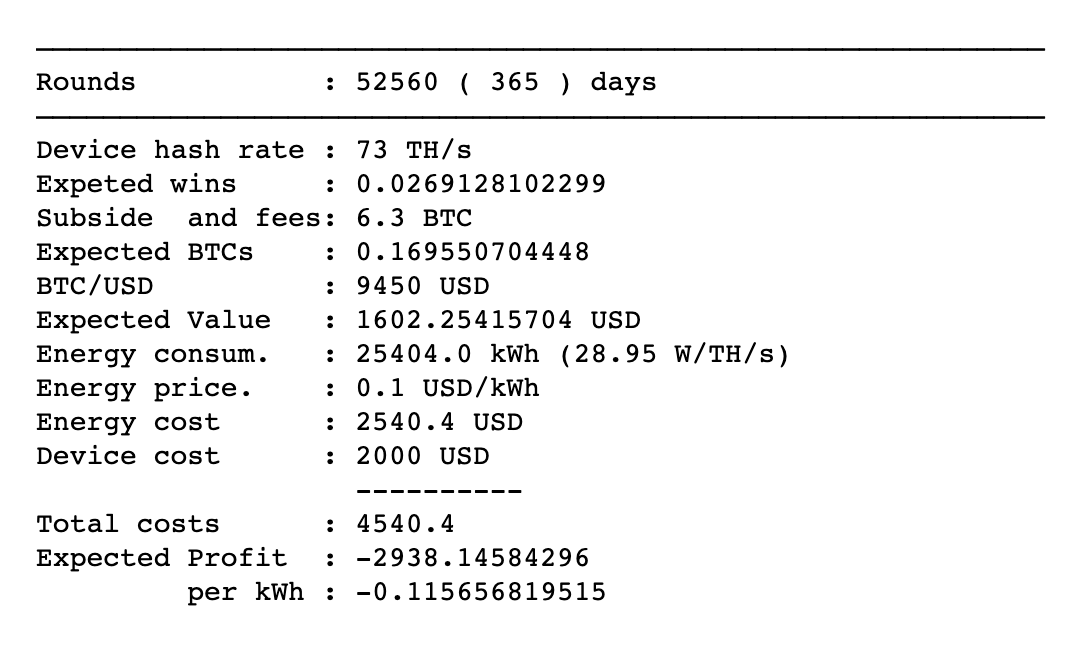
\includegraphics[scale=0.50]{img/results.png}
    \caption{Model results for $S = 6.25 BTC$}
    \label{fig:results}
\end{figure}

\clearpage

\subsection{Simulazione del Processo di Poisson}

In questo paragrafo simuleremo il processo di arrivo di un hash valido in Bitcoin.
Faremo ricorso ad un metodo stocastico.

\begin{equation}
    t = \frac{\ln(1 - U)}{r} \label{generateRandomPoissonProcessNumbers}
\end{equation}

dove $U$ è un numero random corrispondente ad una distribuzione uniforme.

\section{Conclusion}

Many input variables condition the profitability of the mining activity.

For example, the BTC price and fees, the global hash-rate growth, the energy and devices costs, and so on. Further, we should take into account network costs and others.

So, we should refine this method, but it serves as a starting point to debate and improve current public available practices.

This note highlight that within the assumptions and the given costs, solo-mining (or participating in a small pool) is hardly-profitable and poses some questions that we would further investigate:


\begin{itemize}
    \item The cost of electric energy has a high impact on profitability. In which condition we might reduce energy costs?
    \item To take account of other factors that have an impact on the marginal utility (e.g. privacy)
    \item Is the ASIC market overrated? Considering that the devices are not repurposable and the obsolescence rate is very high, the current commercial price seems unjustified.
    \item The system seems to be under the pressure of centralizing forces (both geographically and economically). What will change in the next future? The BTC price? The hash-rate growth? What else? How?
\end{itemize}

With this note, we would give publicity to the fact that the end-user market needs a better model to compute profitability.The proposed method is a point where to start reasoning.

\newpage

\appendix

\section{Blocco}

Le informazioni che riguardano la struttura di un blocco sono contenute nei file bitcoin-core primitives/block.h e primitives/block.cpp.
Come si legge nel file, i nodi verificano e collezionano le transazioni dentro un blocco (con le logiche che vedremo) e ricavano un hash complessivo delle stesse attraverso una struttura dati che prende il nome di albero di Merkle.
Dunque risolvono l'algoritmo di consenso *Proof of Work* che consiste nella ricerca iterativa di un valore nonce `nNonce` da inserire nella testata del blocco (insieme alle altre informazioni) e che dia luogo a un hash di blocco inferiore ad un numero dato che prende il nome di *target*. Il target è collegato alla [difficoltà](./difficolta.md) `nBits`.
Risolto questo algoritmo trasferiscono il blocco agli altri nodi e tutti, se valido, lo inseriscono nella blockchain. La prima transazione del blocco è una transazione speciale che prende il nome di *coinbase*. Si tratta di una transazione che conia moneta a ricompensa del lavoro svolto il nodo che ha trasmesso per primo il nuovo blocco valido. Questa procedura è competitiva: tutti i nodi minatori costruiscoo il blocco destinando la transazione coinbase a un destinatario di loro scelta (in genere il minatore stesso).
> Dopo [SegWit](segregated-witness.md) l'albero di Merkle contiene anche script e firme tramite l'innesto di un sotto-albero per tramite della transazione coinbase.

\section{Rappresentazione difficoltà in Bitcoin}

In Bitcoin, il campo nBits \textbf{codifica} la difficoltà $D$ della Proof of Work del blocco.
Non va confuso con la difficoltà $D$ alla quale è legato dalla relazione (\ref{diff}) che riformulata diviene:

\begin{equation}
    T = \frac{T_{max}}{D} \label{targetFromDiff}
\end{equation}

Il valore \textbf{target} è rappresentato in formato Compat, simile ai numeri in virgola mobile IEEE754, e occupa 32 bit della testata.

\begin{table}[h]
    \centering
    \begin{tabular}{|l|l|l|}
        \hline
        \multicolumn{1}{|c|}{Esponente (b)} & \multicolumn{1}{c|}{Segno (s)} & \multicolumn{1}{c|}{Mantissa (a)} \\ \hline
        8 bit {[}31-24{]}               & 1 bit {[}23{]}             & 23 bits {[}22-00{]}           \\ \hline
    \end{tabular}
\end{table}

Per convertire questo valore in formato intero si utilizza la seguente formula:

\begin{equation}
    T = (-1)^{s} \cdot a \cdot 256^{b}
\end{equation}

\subsection{Conversione da nBits a Target}

La procedura per computare $T$ è la seguente:

\begin{itemize}
    \item ricavare la mantissa tramite i primi 23 bits: nBits \& 0x007fffff
    \item ricavare il segno: nBits \& 0x00800000 != 0
    \item ricavare l'esponente shiftando a destra 24 bit: nBits $\gg$ 24
    \item se $b \le 3$ : translare a destra di $8 \cdot {(3 - b)}$ bit la mantissa
    \item se $b > 3$ : translare a sinistra di $8 \cdot {(b - 3)}$ bit la mantissa
    \item applicare il segno
\end{itemize}


\subsubsection{Esempio}
Ad esempio il valore di nBits del blocco di genesi vale nBits = 0x1d00ffff da cui:
\begin{equation}
    \begin{array}{ll}
        a = \textnormal{0x1d00ffff} \ \& \ \textnormal{0x007fffff} = \textnormal{0xffff} \\
        s = (\textnormal{0x1d00ffff} \ \& \textnormal{0x00800000} != 0) = 0 \\
        b = \textnormal{0x1d00ffff} \gg 24 = \textnormal{0x1d} > 3\\
        a = a << 8 \cdot (b - 3) = \textnormal{0xffff} << \textnormal{0xd0} = \textnormal{0xffff0000000000000000000000000000000000000000000000000000} \\
        a = (-1)^0 \cdot a =  \textnormal{0xffff0000000000000000000000000000000000000000000000000000}
    \end{array}
\end{equation}

Il valore del target massimo, in esadecimale, è il seguente:

$T_{max} = \textit{\scriptsize{0xFFFFFFFFFFFFFFFFFFFFFFFFFFFFFFFFFFFFFFFFFFFFFFFFFFFFFFFF}}$  (56 volte F = $\frac{224}{\ln(16)}$),

che, a causa della rappresentazione compatta, diviene:

$T_{max} = \textit{\scriptsize{0xFFFF0000000000000000000000000000000000000000000000000000}}$ (4 volte F e 52 volte 0).

\subsection{Conversione da Target a nBits}

Il valore nBits è settato dal metodo unsigned int \textit{GetNextWorkRequired()} che,
sotto le opportune condizioni, invoca \textit{GetCompact()}.

Come si vede dal codice sotto riportato si tratta della procedura inversa.

\lstset{style=mystyle}
\begin{lstlisting}[language=c]
// arith_uint256
template <unsigned int BITS>
unsigned int base_uint<BITS>::bits() const
{
    for (int pos = WIDTH - 1; pos >= 0; pos--) {
        if (pn[pos]) {
            for (int nbits = 31; nbits > 0; nbits--) {
                if (pn[pos] & 1U << nbits)
                    return 32 * pos + nbits + 1;
            }
            return 32 * pos + 1;
        }
    }
    return 0;
}

uint32_t arith_uint256::GetCompact(bool fNegative) const
{
    int nSize = (bits() + 7) / 8;
    uint32_t nCompact = 0;
    if (nSize <= 3) {
        nCompact = GetLow64() << 8 * (3 - nSize); // qui viene impostata la mantissa
    } else {
        arith_uint256 bn = *this >> 8 * (nSize - 3);
        nCompact = bn.GetLow64(); // qui viene impostata la mantissa
    }
    // The 0x00800000 bit denotes the sign.
    // Thus, if it is already set, divide the mantissa by 256 and increase the exponent.
    if (nCompact & 0x00800000) {
        nCompact >>= 8;
        nSize++;
    }
    assert((nCompact & ~0x007fffff) == 0);
    assert(nSize < 256);
    nCompact |= nSize << 24; // qui viene impostato l'esponente
    nCompact |= (fNegative && (nCompact & 0x007fffff) ? 0x00800000 : 0); // qui viene impostato il segno
    return nCompact;
}
\end{lstlisting}

\section{Proof of Work}

Bitcoin-core esegue la PoW in mining.cpp all'interno della funzione generateBlocks.

\lstset{style=mystyle}
\begin{lstlisting}[language=c]
// permette di inizializzare il nuovo blocco prima della PoW con
void IncrementExtraNonce(CBlock* pblock, const CBlockIndex* pindexPrev, unsigned int& nExtraNonce)
{
  //...
}
\end{lstlisting}

Poi con un ciclo while viene modificato solo il nounce

\lstset{style=mystyle}
\begin{lstlisting}[language=c]
while (nMaxTries > 0 && pblock->nNonce < std::numeric_limits<uint32_t>::max() && !CheckProofOfWork(pblock->GetHash(), pblock->nBits, Params().GetConsensus()) && !ShutdownRequested()) {
    ++pblock->nNonce; // qui
    --nMaxTries;
}
\end{lstlisting}

GetNextWorkRequired è chiamata da UpdateTime chiamato da CreateNewBlock
In maniera analogo dobbiamo modificare la PoW per evitare di inizializzare i dati ad ogni step.
In analogia sposterò generateBlock in mining. Al momento MineTx in Network

\newpage

\bibliographystyle{plain}
\bibliography{references}

\end{document}